\chapter{Perancangan}
\label{chap:design}

Pada bab ini akan dipaparkan berbagai macam rancangan dari perkakas \cl yang akan dibuat, seperti diagram-diagram terkait, masukan serta keluaran perangkat lunak,
% Jangan lupa - bagian ini belum selesai!

\section{Rancangan Diagram}
\label{sec:design-diagrams}

Bagian ini akan membahas mengenai alur dari \textit{activity diagram} serta \textit{sequence diagram} dari perkakas yang akan dibuat. Perlu diingat bahwa perkakas yang akan dibuat memiliki tiga buah fitur, yaitu:

\begin{itemize}
	\item mencari lokasi menggunakan kata kunci pencarian (\verb|searchplace|),
	\item mencari rute dengan angkot menggunakan \latlon lokasi (\verb|findroute|), dan
	\item mencari rute dengan angkot menggunakan kata kunci pencarian lokasi (\verb|direct|).
\end{itemize}

\noindent
Oleh karena itu, tiap-tiap fitur akan memiliki satu dari setiap tipe diagram. Adapun penjelasan dari bagaimana fitur-fitur ini akan diimplementasikan adalah sebagai berikut.

% Tambahkan deskripsi jika diagram kelas dibuat!!

\subsection{Mencari lokasi menggunakan kata kunci pencarian}
\label{sec:design-diagrams-searchplace}

\begin{figure}[ht]
    \centering
    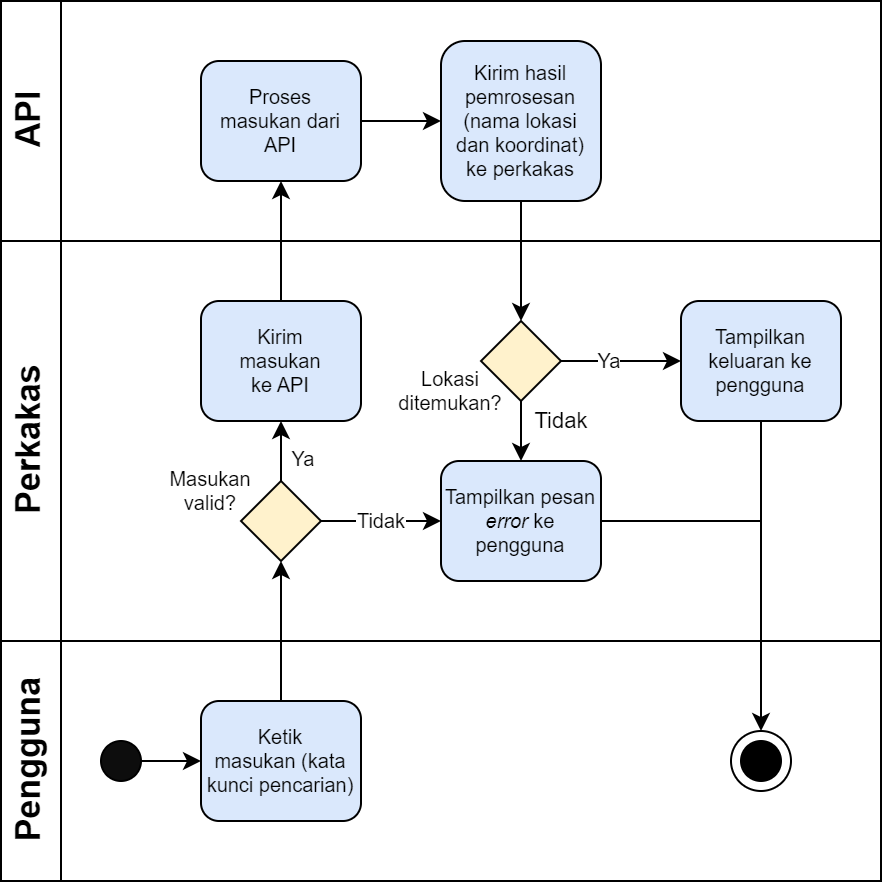
\includegraphics[width=0.55\linewidth]{diagrams-activity-searchplace}
    \caption[Diagram \textit{use case} perkakas yang akan dibangun]{\textit{Activity diagram} dari fitur pencarian lokasi menggunakan kata kunci pencarian.}
    \label{fig:diagrams-activity-searchplace}
\end{figure}

\begin{figure}[ht]
    \centering
    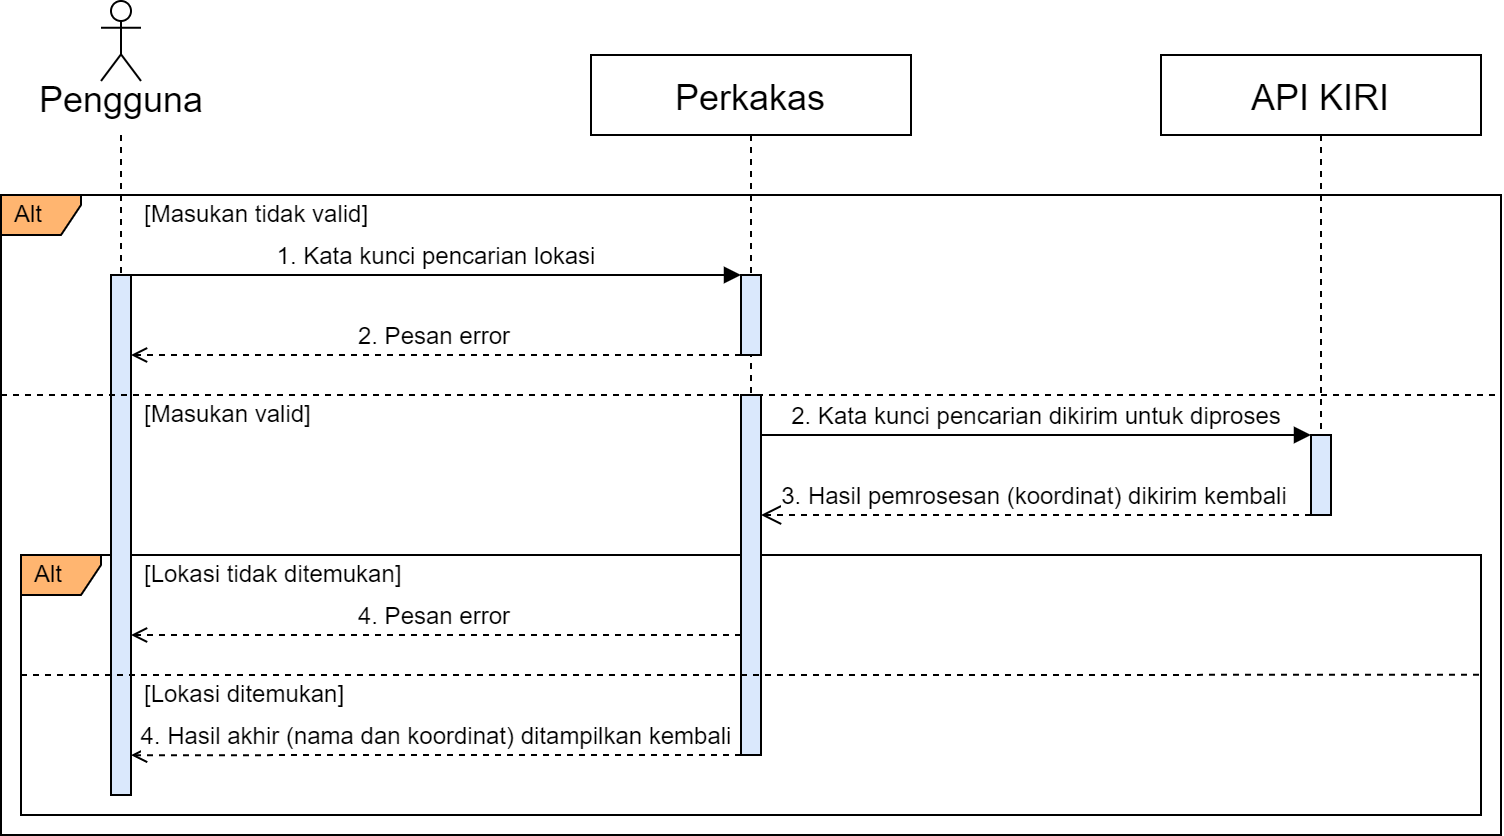
\includegraphics[width=0.8\linewidth]{diagrams-sequence-searchplace}
    \caption[Diagram \textit{use case} perkakas yang akan dibangun]{\textit{Sequence diagram} dari fitur pencarian lokasi menggunakan kata kunci pencarian.}
    \label{fig:diagrams-sequence-searchplace}
\end{figure}

Detail dari alur diagram untuk fitur ini adalah sebagai berikut.

\begin{enumerate}
	\item Perkakas akan meminta masukan dari pengguna berupa kata kunci dari lokasi yang ingin dicari.
	\item Masukan akan dicek oleh perkakas validitasnya. Dalam kasus ini, masukan hanya akan dianggap tidak valid apabila pengguna tidak memasukkan apapun sebagai masukan perkakas (masukan kosong).
	\item Jika kata kunci masukan:

	\begin{itemize}
		\item tidak valid, maka perkakas akan mengeluarkan pesan \textit{error} dan keluar.
		\item dianggap valid, kata kunci tersebut akan dikirim ke API KIRI untuk diproses lebih lanjut.
	\end{itemize}
	
	\item Setelah selesai diproses, keluaran dari API akan dikembalikan ke perkakas.
	\item Perkakas akan mengecek keluaran yang diterimanya. Apabila lokasi:
	
	\begin{itemize}
		\item ditemukan, maka nama dan koordinat \latlon lokasi akan ditampilkan ke pengguna sebagai keluaran akhir.
		\item tidak ditemukan, maka perkakas akan mengeluarkan pesan \textit{error} dan keluar.
	\end{itemize}
	
	Perlu diingat bahwa perkakas tidak peduli apakah lokasi yang ditemukan benar (sesuai dengan yang diinginkan pengguna) atau tidak.
	
\end{enumerate}

\subsection{Mencari rute dengan angkot menggunakan \latlon lokasi}
\label{sec:design-diagrams-findroute}

\begin{figure}[ht]
    \centering
    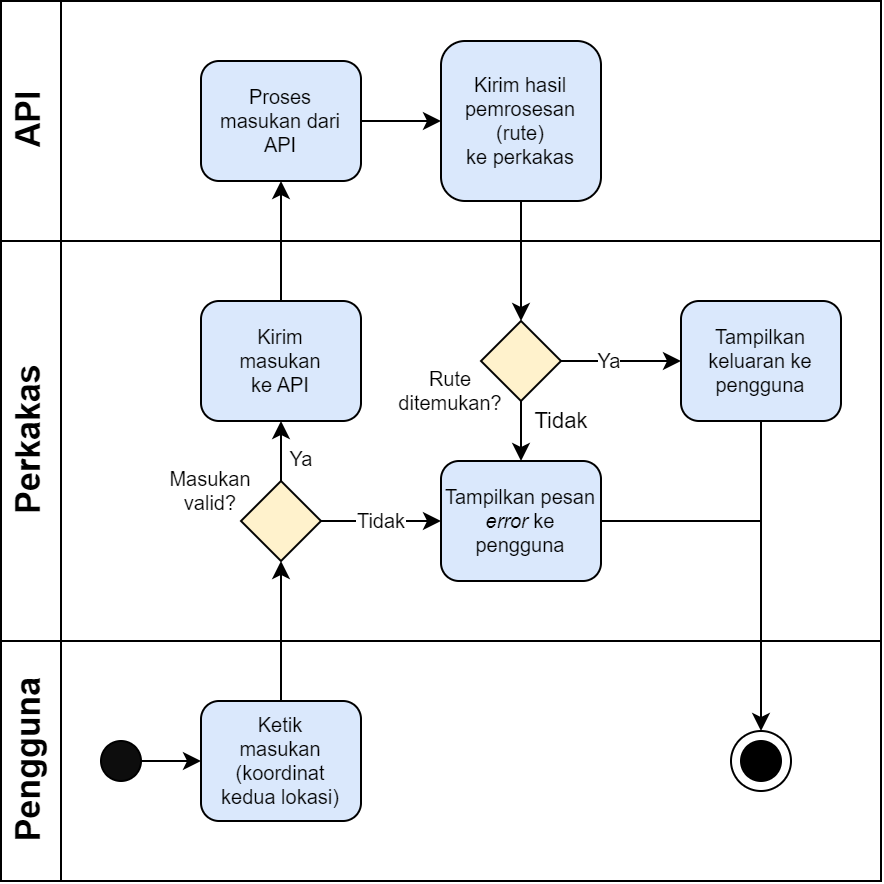
\includegraphics[width=0.55\linewidth]{diagrams-activity-findroute}
    \caption[Diagram \textit{use case} perkakas yang akan dibangun]{\textit{Activity diagram} dari fitur pencarian rute angkot menggunakan \latlon lokasi.}
    \label{fig:diagrams-activity-findroute}
\end{figure}

\begin{figure}[ht]
    \centering
    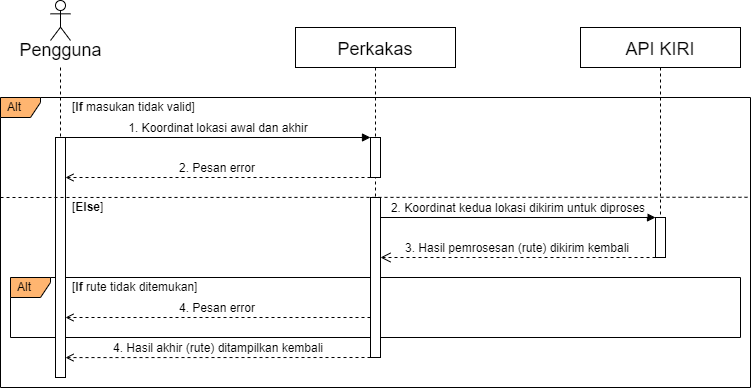
\includegraphics[width=0.8\linewidth]{diagrams-sequence-findroute}
    \caption[Diagram \textit{use case} perkakas yang akan dibangun]{\textit{Sequence diagram} dari fitur pencarian rute angkot menggunakan \latlon lokasi.}
    \label{fig:diagrams-sequence-findroute}
\end{figure}

Detail dari alur diagram untuk fitur ini adalah sebagai berikut.

\begin{enumerate}
	\item Perkakas akan meminta dua buah masukan dari pengguna, berupa koordinat \latlon dari lokasi awal (mulai) dan lokasi akhir (tujuan).
	\item Masukan akan dicek oleh perkakas validitasnya. Dalam kasus ini, masukan akan dianggap tidak valid apabila ada masukan yang bukan berupa koordinat \latlon .
	\item Jika:
	
	\begin{itemize}
		\item satu atau lebih masukan tidak valid, maka perkakas akan mengeluarkan pesan \textit{error} dan keluar.
		\item kedua masukan dianggap valid, kedua koordinat tersebut akan dikirim ke API KIRI untuk diproses lebih lanjut.
	\end{itemize}
	 
	\item Setelah selesai diproses, keluaran dari API akan dikembalikan ke perkakas.
	\item Perkakas akan mengecek keluaran yang diterimanya. Apabila rute:
	
	\begin{itemize}
		\item berhasil ditemukan (ada setidaknya satu langkah dalam rute), maka rute tersebut akan ditampilkan ke pengguna sebagai keluaran akhir.
		\item tidak berhasil ditemukan, maka perkakas akan mengeluarkan pesan \textit{error} dan keluar.
	\end{itemize}
	
\end{enumerate}

\subsection{Mencari rute dengan angkot menggunakan kata kunci pencarian lokasi}
\label{sec:design-diagrams-direct}

\begin{figure}[ht]
    \centering
    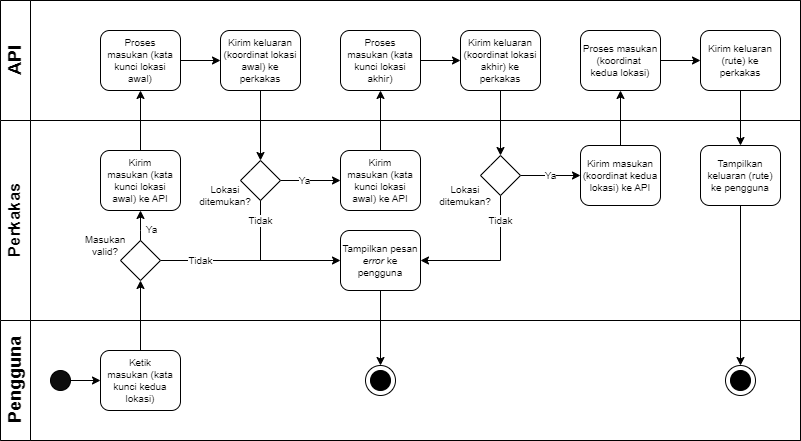
\includegraphics[width=\linewidth]{diagrams-activity-direct}
    \caption[Diagram \textit{use case} perkakas yang akan dibangun]{\textit{Activity diagram} dari fitur pencarian rute angkot menggunakan kata kunci pencarian.}
    \label{fig:diagrams-activity-direct}
\end{figure}

\begin{figure}[ht]
    \centering
    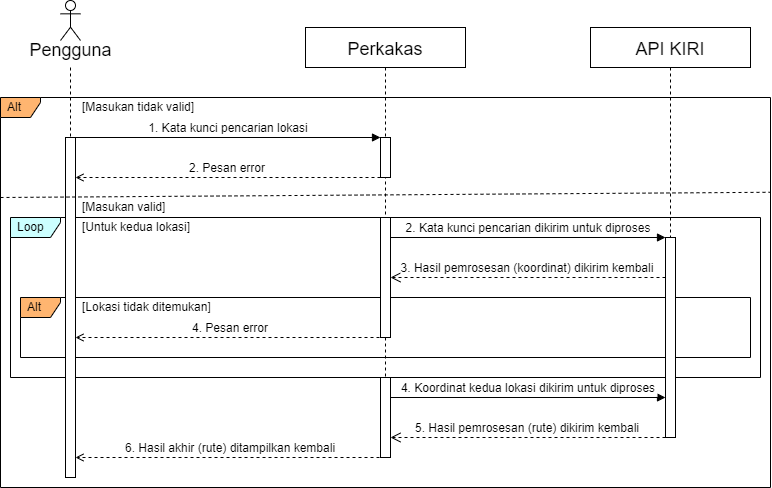
\includegraphics[width=0.8\linewidth]{diagrams-sequence-direct}
    \caption[Diagram \textit{use case} perkakas yang akan dibangun]{\textit{Sequence diagram} dari fitur pencarian rute angkot menggunakan kata kunci pencarian.}
    \label{fig:diagrams-sequence-direct}
\end{figure}

Detail dari alur diagram untuk fitur ini adalah sebagai berikut.

\begin{enumerate}
	\item Perkakas akan meminta masukan dari pengguna berupa kata kunci dari lokasi awal dan lokasi akhir yang ingin dicari.
	\item Masukan untuk lokasi awal akan dicek oleh perkakas validitasnya. Dalam kasus ini, masukan hanya akan dianggap tidak valid apabila pengguna tidak memasukkan apapun (masukan kosong), atau memasukkan koordinat \latlon sebagai masukan perkakas.
	\item Jika kata kunci masukan:
	
	\begin{itemize}
		\item tidak valid, maka perkakas akan mengeluarkan pesan \textit{error} dan keluar.
		\item dianggap valid, kata kunci tersebut akan dikirim ke API KIRI untuk diproses lebih lanjut.
	\end{itemize}
	 
	\item Setelah selesai diproses, keluaran dari API akan dikembalikan ke perkakas.
	\item Perkakas akan mengecek keluaran yang diterimanya. Apabila lokasi:
	
	\begin{itemize}
		\item tidak ditemukan, maka perkakas akan mengeluarkan pesan \textit{error} dan keluar.
		\item ditemukan, maka nama dan koordinat \latlon lokasi awal akan disimpan sebagai variabel untuk dipakai di langkah selanjutnya.
	\end{itemize}
	
	\item Langkah 2 sampai 5 akan diulang kembali untuk lokasi akhir.
	\item Jika kata kunci kedua lokasi berhasil diproses, perkakas akan mengirim kembali koordinat \latlon dari kedua lokasi tersebut ke API sebagai masukan untuk proses kedua, yaitu mencari rute angkot dengan koordinat \latlon lokasi.
	\item Setelah selesai diproses, keluaran berupa rute dari API akan dikembalikan ke perkakas.
	\item Perkakas akan mengecek keluaran yang diterimanya. Apabila rute:
	
	\begin{itemize}
		\item berhasil ditemukan (ada setidaknya satu langkah dalam rute), maka rute tersebut akan ditampilkan ke pengguna sebagai keluaran akhir.
		\item tidak berhasil ditemukan, maka perkakas akan mengeluarkan pesan \textit{error} dan keluar.
	\end{itemize}
	
\end{enumerate}
